\begin{figure}[h] 
\centering 
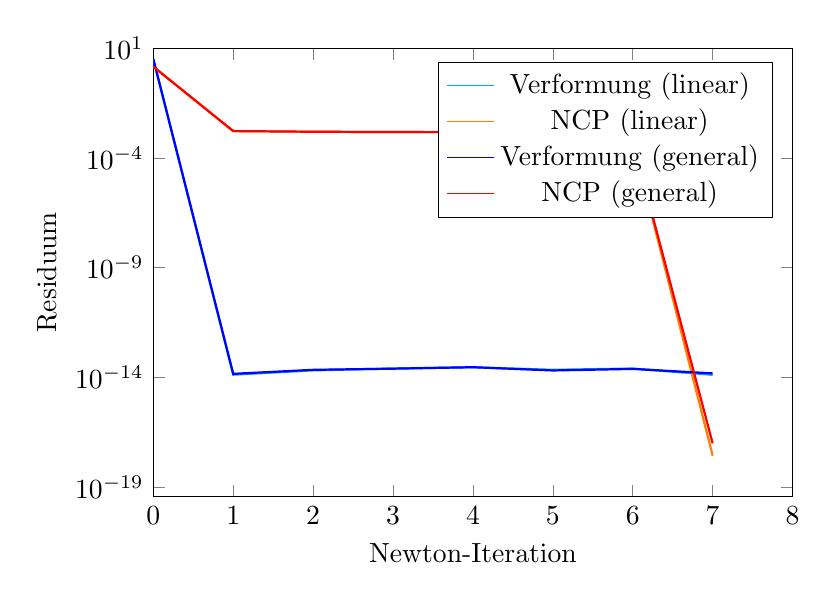
\begin{tikzpicture}[every plot/.append style={thick}] 
\begin{axis}[ 
label style={font=\normalsize}, 
xlabel={Newton-Iteration}, 
ylabel={Residuum}, 
xmin=0, xmax=8, 
ymode=log, 
ymin=0, ymax=10, 
width=0.8\textwidth, 
height=0.6\textwidth, 
legend pos=north east, 
legend style={cells={align=left}}, 
grid style=dashed, 
] 
\addplot[ 
color=cyan, 
] 
coordinates { 
(0, 3.20e+00)(1, 1.31e-14)(2, 2.06e-14)(3, 2.52e-14)(4, 2.85e-14)(5, 2.18e-14)(6, 2.50e-14)(7, 1.29e-14)}; 
\addlegendentry{Verformung (linear)} 
\addplot[ 
color=orange, 
] 
coordinates { 
(0, 1.43e+00)(1, 1.66e-03)(2, 1.55e-03)(3, 1.50e-03)(4, 1.48e-03)(5, 1.05e-03)(6, 5.93e-04)(7, 2.65e-18)}; 
\addlegendentry{NCP (linear)} 
\addplot[ 
color=blue, 
] 
coordinates { 
(0, 3.20e+00)(1, 1.43e-14)(2, 2.18e-14)(3, 2.46e-14)(4, 2.87e-14)(5, 2.04e-14)(6, 2.40e-14)(7, 1.50e-14)}; 
\addlegendentry{Verformung (general)} 
\addplot[ 
color=red, 
] 
coordinates { 
(0, 1.43e+00)(1, 1.66e-03)(2, 1.55e-03)(3, 1.50e-03)(4, 1.48e-03)(5, 1.05e-03)(6, 5.93e-04)(7, 9.68e-18)}; 
\addlegendentry{NCP (general)} 
\end{axis} 
\end{tikzpicture} 
\caption{Residuen des Stoffgesetzes 'Linear elastisch' mit Hinderniss 'Spitze' und 578 Freiheitsgraden für die Verschiebung.} 
\label{fiq:Linearelastisch_Spitze_level3} 
\end{figure} 
